In order to obtain sufficient labeled training data and make experiments efficient and repeatable to study the proposed RCA system, 
we created a high-fidelity emulation environment in the NSF ExoGENI cloud testbed~\cite{ExoGENI:web} that can automatically create a virtual network system with virtual machines (VMs), bootstrap the network routing, 
initiate data transfers, inject arbitrary integrity errors into the virtual router interfaces and end hosts, and collect training data.

To inject controlled errors into any network elements, we added a new utility in Chaos Jungle~\cite{swip:pearc:2019,chaosjungle:web}, which can corrupt arbitrary file(s) in nodes in addition to packets out of network interfaces according to a given probability. In this way, labeled data can be generated to train the machine learning models. 

At the last step, all the raw data will be processed and stored in the final result database files with predefined feature columns. Each database entry represents one data transfer with features of the file name, file size, origin, sink, access router, integrity error or not, etc. However, the forwarding path is unknown as it is controlled by the routing control plane process. The final result is exported to a Jupyter notebook environment where all the ML-based data analysis is performed.


\begin{figure}[!ht]
\begin{center}
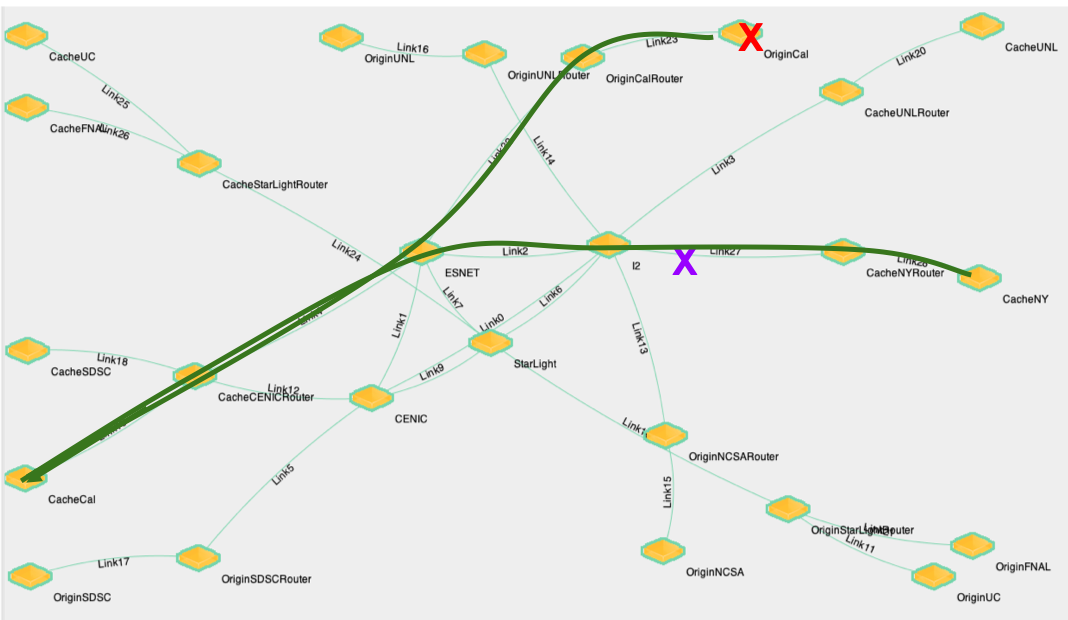
\includegraphics[width=0.48\textwidth]{./figure/ChaosJungle}
\end{center}
\caption{Fault Injection in an Emulated Network}
\label{fig:topology}
\vspace{-0.1in}
\end{figure}

We use Fig. 2, an annotated screenshot from the ExoGENI GUI, to illustrate an emulated network system, a simplified version of the Open Science Grid (OSG) data federation network, a highly utilized wide area network to distribute data for high throughput scientific computing~\cite{OSG:web}. This network consists of multiple end hosts running the data transfer and computing jobs controlled by Pegasus WMS~\cite{deelman-fgcs-2015}, and a set of routers in the middle to represent multiple forwarding domains. The unit of data transfers is a {\it file} of different size for which we define as a {\it flow} from an origin end host to a destination end host. The two cross signs, one on an 
end host and another one on a network link, represent the locations where we inject the data integrity errors with a probability setting. When an error is enabled (injected), all the traffic flows that pass through the faulty element will be subject to possible data corruption as the error may flip the bits of packets randomly under a predefined probability. As we have discussed, most of these corrupted packets will not be caught by TCP or the storage system. As a result, some corrupted files will successfully land at the destination end hosts and will only be detected by Pegasus at the application layer. 

This emulation environment can be used to create a sandbox to generate high-fidelity RCA models for a production networked system. 